\begin{figure*}[t]
\centering
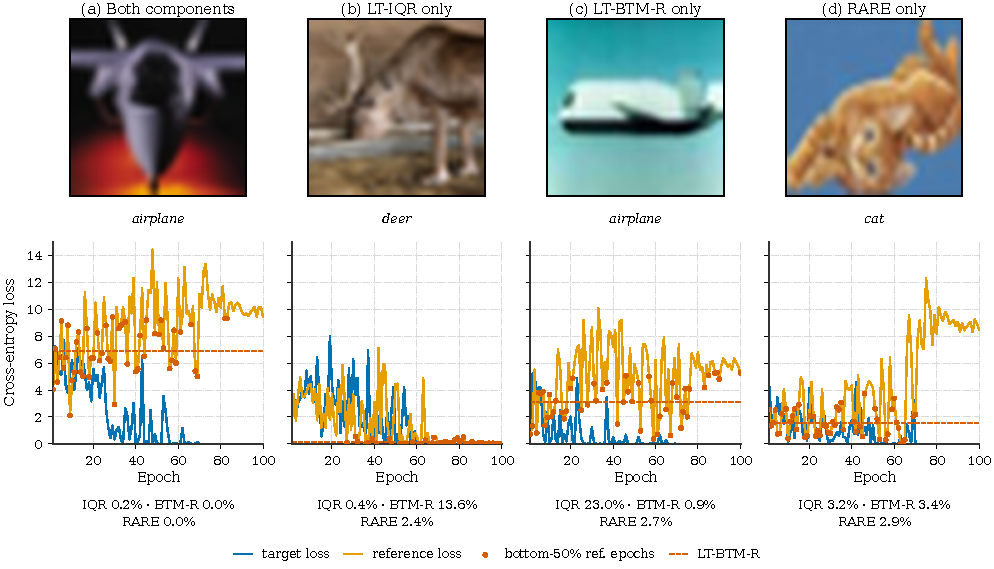
\includegraphics[width=0.75\textwidth]{figures/fig_qualitative_examples.pdf}
\caption{
Four CIFAR10 members flagged as vulnerable by LiRA-256 at
FPR$=10^{-4}$ (WRN-28-2 target). Per-epoch target (blue) and
single-reference (orange) losses; dots mark the reference's
bottom-$50\%$ checkpoints, whose mean defines LT-BTM-R (dashed).
Lower percentages indicate more vulnerability
({\em e.g.} 1\% means among the top 1\% of vulnerability ranks). 
Panels show, in turn, a member recovered by both
components~(a), by target-side LT-IQR only~(b), by reference-side
LT-BTM-R only~(c), and by neither component alone but by their standardized
sum~(d).
}
\label{fig:qualitative_examples}
\end{figure*}
